\apendice{Documentación de usuario}

\section{Introducción}
En este apartado se explicarán los pasos necesarios para poder instalar la aplicación y usarla correctamente.

\section{Requisitos de usuarios}
\begin{itemize}
    \item Es necesario disponer de un sistema operativo Windows 7 o superior o Ubuntu 16.04 LTS\footnote{Pueden usarse otras distribuciones Linux, pero los ficheros de instalación proporcionados pueden no funcionar}.

    \item El procesador del equipo puede ser de 32 o 64 bits.

    \item En cuanto al software, será necesario tener instalado en el equipo Java 8 y Python 3.
\end{itemize}


\subsection{Sistemas Windows}
Para Windows descargaremos Java 8 desde:\\ \url{http://www.oracle.com/technetwork/java/javase/downloads/}

Para obtener Python 3, descargaremos la siguiente versión de Miniconda3\footnote{Actualmente existen errores en los repositorios de \textit{conda} al instalar la última versión de Miniconda3, pero en la versión que aquí se facilita, la instalación es correcta.}:
\begin{itemize}
    \item Si nuestro sistema es de 32 bits:\\ \url{https://repo.continuum.io/miniconda/Miniconda3-3.19.0-Windows-x86.exe}
    \item Si nuestro sistema es de 64 bits:\\ \url{https://repo.continuum.io/miniconda/Miniconda3-3.19.0-Windows-x86_64.exe}
\end{itemize}
Al instalar Miniconda3 hay que marcar la opción de añadir Anaconda al \textit{path} del sistema como en la figura \ref{fig:img/ManualUsuario/Miniconda}.

\imagen{img/ManualUsuario/Miniconda}{Instalación de Miniconda}


\subsection{Sistemas Linux}
La instalación de Java 8 para sistemas Linux se debe llevar a cabo desde una terminal mediante el siguiente comando:\\
\centerline{\textit{\$ sudo apt-get install oracle-java8-installer}}

Python 3 viene incluido desde hace tiempo en las distribuciones Linux ya que, en un futuro, será la versión por defecto. En caso de que no estuviese instalado utilizaríamos el siguiente comando desde una terminal: \\
\centerline{\textit{\$ sudo apt-get install python3}}

\newpage
\section{Instalación}
Una vez cumplidos con los requisitos, descargaremos el fichero \textit{Perikymata2.0.zip}, que contiene la última versión disponible de la aplicación. Podemos encontrarlo en el siguiente enlace: \\\url{https://github.com/amtBurgos/Perikymata2017/releases} 

En el encontraremos cuatro elementos:
\begin{itemize}
    \item La aplicación Java llamada \textit{Perikymata2.0.jar}.
    \item La carpeta con el servidor en Python llamada \textit{PythonApp}.
    \item Un script Linux llamado \textit{StartPerikymata.sh}\footnote{Ha sido necesario incluir este fichero porque, mediante el doble clic, el arranque de la aplicación no respondía adecuadamente.} para arrancar la aplicación Java.
    \item Una carpeta llamada \textit{Installation} con los scripts para poder instalar \textit{Scikit-Image} en Windows y Linux.
\end{itemize}

Será necesario instalar \textit{Scikit-Image} para que funcione el servidor de Python por lo que se han incluido en la carpeta \textit{Installation} dos ficheros:
\begin{itemize}
    \item Para instalar \textit{Scikit-Image} en Windows, haremos doble clic sobre \textit{ServerInstallation.bat} y esperaremos, ya que el proceso tarda un rato.
    \item Para instalarlo en Linux, abriremos una terminal desde la carpeta \textit{Installation} y ejecutaremos los siguientes comandos:
    
    \centerline{\textit{\$ chmod +x ServerInstallationLinux.sh}\footnote{Este comando da permisos de ejecución al script.}}
    \\ \centerline{\textit{\$ ./ServerInstallationLinux.sh}\footnote{Es posible que nos pida alguna confirmación para realizar la instalación.}}
    
    La distribución donde se han probado estos \textit{scripts} es Ubuntu 16.04 LTS. Es posible que no funcionen en otras distribuciones, en tal caso, correrá a cuenta del usuario instalar \textit{Scikit-Image} y sus dependencias. Podemos encontrar los pasos desde su página oficial: \\ \url{http://scikit-image.org/docs/0.13.x/install.html}
    
    Dejaremos preparado también, los permisos del fichero \textit{StartPerikymata.sh}, abriendo una terminal desde la carpeta principal \textit{Perikymata2.0} e introduciendo el siguiente comando: \\
    \centerline{\textit{\$ chmod +x StartPerikymata.sh}}
\end{itemize}

\newpage
\section{Manual del usuario}

A continuación se mostrará el modo de usar la aplicación, explicando cada una de sus fases, opciones y el flujo normal de ejecución. Las fases que contiene son las siguiente:
\begin{itemize}
    \item Arranque de la aplicación. En esta fase se crea o se abre un proyecto.
    \item Selección y unión de imágenes (\textit{stitching}). Se juntan las imágenes para conseguir una imagen completa de la pieza dental.
    \item Rotación y recortado de la imagen. Se prepara la imagen para el filtrado y se consigue la medida.
    \item Filtrado de la imagen. Se filtra la imagen para marcar las perikymata.
    \item Marcado de perikymata y exportación de datos.
\end{itemize}

\subsection{Arranque de la aplicación}
En primer lugar, es necesario recordar que para que la aplicación funcione, deben estar en la misma carpeta el ejecutable Java y la carpeta con el servidor de Python. 

Como veíamos en la sección anterior, la carpeta \textit{Perikymata2.0} tiene dos elementos, el servidor en Python (carpeta \textit{PythonApp}) y el ejecutable Java de la aplicación principal (\textit{Perikymata2.0.jar}).

Desde esa carpeta, en Windows haremos doble clic sobre el fichero \textit{Perikymata2.0.jar} y en Linux abriremos una terminal y pondremos el siguiente comando: \\ \centerline{\textit{\$ ./StartPerikymata.sh}}

Este script ejecuta el comando: \textit{\$ java -jar Perikymata2.0.jar}. Ha sido necesario incluir este fichero en Linux debido a que el doble clic no funcionaba en algunas ocasiones, así nos aseguramos de que la aplicación se inicia correctamente siempre\footnote{La aplicación en Linux puede dar a veces errores que causan el mal funcionamiento de la botonera superior y el redimensionado de la aplicación}.  

Automáticamente se inicia el servidor, la primera vez que se ejecute todo el proyecto puede tardar un poco en arrancar porque necesita crear unos archivos en caché, por lo que esperaremos. En Linux corre en segundo plano, pero en Windows se nos abre una ventana de comandos donde veremos las operaciones que van sucediendo. 

\newpage
Si no teníamos ningún proyecto cargado, aparecerá la primera ventana de la aplicación como la de la figura \ref{fig:img/ManualUsuario/FaseInicio}. En caso contrario, se abrirá el último proyecto con el que se ha trabajado desde la última etapa de la aplicación donde se tengan datos.

\imagenDos{img/ManualUsuario/FaseInicio}{Fase de inicio}{1}

En esta ventana encontraremos tres botones:
\begin{itemize}
    \item \textit{New Project}: crea un nuevo proyecto de perikymata, para ello nos pide el nombre y el lugar donde queremos guardarlo.
    \item \textit{Open Project}: Abre un proyecto. Tenemos que buscar la carpeta del proyecto que queremos abrir y en ella, el fichero XML que contiene la configuración. El nombre de este fichero es del tipo \textit{<NombreProyecto>.xml}. 
    \item \textit{Cancel}: Cierra el servidor y la aplicación.
\end{itemize}

Pulsaremos \textit{New Project} y crearemos un proyecto en un sitio de nuestra preferencia. Dentro del proyecto, se crearán los siguientes elementos:
\begin{itemize}
    \item Carpeta \textit{Fragments}: contiene los fragmentos que se han seleccionado para juntar las imágenes en la fase de selección y unión de imágenes.
    \item Carpeta \textit{Full\_Image}: contiene la imagen completa del diente, que ha introducido el usuario o que es el resultado de la unión de los fragmentos
    \item Carpeta \textit{Cropped\_Image}: Contiene la imagen original recortada de la fase de recorte, la imagen filtrada con líneas detectadas y la imagen original con las líneas detectadas superpuestas.
    \item Carpeta \textit{Perikymata\_Outputs}: contiene el fichero \textit{csv} con los datos exportados.
    \item Fichero \textit{\textit{<NombreProyecto>.xml}}: es el fichero de configuración del proyecto. Contiene información sobre la carpeta temporal elegida, las líneas dibujadas y las perikymata marcadas.
\end{itemize}

\subsection{Selección y unión de imágenes}

La siguiente fase es la selección y unión de imágenes. La pantalla que nos aparecerá es como la de la figura \ref{fig:img/ManualUsuario/FaseStitching}

\imagenDos{img/ManualUsuario/FaseStitching}{Fase de selección y unión de imágenes}{1}

El objetivo es tener la imagen completa del diente. Los pasos para obtenerla serán los siguientes:
\begin{itemize}
    \item Pulsar \textit{Load image pieces}: nos permitirá cargar las imágenes de fragmentos del diente.
    \item Pulsar \textit{Delete from list}: si nos hemos equivocado, seleccionaremos la imagen a borrar de la lista y luego pulsaremos este botón.
    \item Pulsar \textit{Generate full image}: inicia el proceso de unión de imágenes \textit{stitching}. Tarda más tiempo o menos dependiendo de la cantidad de imágenes y de la potencia del ordenador.
    \item Pulsar \textit{Load full image}: con este botón cargamos una imagen completa del diente que tengamos. En este caso no haría falta cargar y unir los fragmentos pequeños.
    \item Pulsar \textit{Rotate 90º}: la imagen tiene que estar con las perikymata orientadas verticalmente. Este botón nos permite rotar la imagen de forma rápida.
    \item Pulsar \textit{Save project and continue}: guarda las imágenes y pasa a la siguiente fase.
\end{itemize}

En la figura \ref{fig:img/ManualUsuario/FaseStitching} también vemos un elemento en la parte de abajo, las \textit{migas de pan}. Nos permiten ver en que fase de la aplicación nos encontramos y retroceder a otras anteriores.


\subsection{Rotación y recortado de la imagen}
En esta fase, el objetivo es rotar y recortar en la imagen la zona de la corona, para que la aplicación pueda más adelante delimitar bien los deciles donde se encuentran las perikymata. 

También se busca dejar las perikymata orientadas los más verticalmente posible y para ello se permite rotar la imagen en un ángulo de 40º hacia cada lado. Además en esta fase, también se guarda la medida de la imagen que permite saber la escala.

Los botones tienen \textit{tooltips}, de modo que si dejamos el ratón encima, nos aparecerá un mensaje explicando para que vale cada botón.

Podemos ver la rotación y recortado en la figura \ref{fig:img/ManualUsuario/FaseRotacion}.
\imagenDos{img/ManualUsuario/FaseRotacion}{Fase de rotación y recortado de la imagen}{1.02}

En primer lugar, usaremos el \textit{slider} para rotar la imagen. También podemos introducir los grados que queremos que gire; para girar hacia la derecha introduciremos números positivos y hacia la izquierda, negativos.

Después con el botón \textit{cuadrado} seleccionaremos la zona de la corona en la imagen y con el botón \textit{recorte}\footnote{El recorte debe hacerse desde la parte izquierda de la imagen hacia la derecha.} recortaremos la imagen. Esa imagen recortada será la que filtremos y sobre la que marquemos las perikymata. Es importante que el recorte abarque la anchura de la corona porque es donde se marcarán los deciles. La altura que debe tener el recorte queda a criterio del usuario; si damos más altura puede que incluyamos zonas de las perikymata que se vean y detecten mejor. Cuando más grande sea el recorte, más tiempo tardará en filtrarse (dentro de un tiempo razonado).

Si no estamos satisfechos con el recorte pulsaremos sobre \textit{Reset View} para desechar los cambios.
 
Para obtener la medida pulsaremos en \textit{Measure Line}. Después, pulsaremos y arrastraremos sobre la imagen en la zona de la leyenda para dibujar una línea roja que abarque la medida. Cuando acabemos, aparecerá una ventana donde nos pide ingresar la unidad de la medida (cm, mm, nm, etc) y el valor (figura \ref{fig:img/ManualUsuario/FaseMedida}). Estos datos podemos cambiarlos también con el botón \textit{Measure Unit and Value}.
\imagenDos{img/ManualUsuario/FaseMedida}{Medida de la imagen}{0.85}

Para concluir esta fase, pulsaremos sobre \textit{Save all and Continue}, se guardaran todos los datos y se pasará a la fase de filtrado y recuento de perikymata.

\subsection{Filtrado de la imagen}
El servidor en Python nos da el servicio de filtrado, en Windows se puede ver en la ventana de comandos que tenemos junto a la aplicación y en Linux corre en segundo plano.



En esta fase filtraremos la imagen\footnote{El servidor tiene que estar arrancado, en caso contrario aparecerán mensajes de que no se puede filtrar} para marcar las perikymata y que después se puedan marcar fácilmente. Para ello contamos con el modo por defecto y modo avanzado. El estado inicial de la ventana será como el de la figura \ref{fig:img/ManualUsuario/FaseFiltrado1}

\imagenDos{img/ManualUsuario/FaseFiltrado1}{Estado inicial de la ventana de filtrado y recuento}{1}


Para usar el modo por defecto, solamente pulsaremos el botón \textit{Filter} y esperaremos hasta que la imagen cambie a una como en la figura \ref{fig:img/ManualUsuario/FaseFiltrado2}. Esta imagen está filtrada, con las perikymata encontradas reducidas a una anchura de un píxel, en color blanco, y las partes detectadas con línea roja.
\imagenDos{img/ManualUsuario/FaseFiltrado2}{Imagen filtrada por defecto}{1}

Disponemos de un botón \textit{Alternate View} para cambiar a la imagen original con las líneas detectadas superpuestas, como en la figura \ref{fig:img/ManualUsuario/FaseFiltrado3}.
\imagenDos{img/ManualUsuario/FaseFiltrado3}{Imagen original con líneas superpuestas}{1}

Aunque el filtrado por defecto es efectivo, con el filtrado avanzado tendremos más control para que se detecten mejor las perikymata. Pulsaremos el botón \textit{Advanced Fiilter} y se extenderá la parte izquierda mostrando los parámetros del filtrado que podemos modificar (figura \ref{fig:img/ManualUsuario/FaseFiltrado4}).
\imagenDos{img/ManualUsuario/FaseFiltrado4}{Filtrado avanzado}{1}

Explicaremos a continuación para que sirven cada uno de estos parámetros:
\begin{itemize}
    \item \textit{Enable lines detection}: si lo dejamos marcado, podremos modificar parámetros hasta la opción \textit{Max detection angle} (incluido) y en la imagen se reducirán perikymata a una anchura de un píxel (color blanco) y luego se detectarán las líneas (color rojo). Si lo desmarcamos, solo podremos modificar las dos últimas opciones y el resultado será una imagen con las perikymata reducidas a un píxel marcadas de color rojo, sin detección de líneas.\\Se recomienda desactivarlo si en la imagen original, las perikymata, se ven muy bien, pero si no se aprecian bien es mejor marcarlo. Podemos ver el resultado sin marcar en la figura \ref{fig:img/ManualUsuario/FaseFiltrado5}. 
    \imagenDos{img/ManualUsuario/FaseFiltrado5}{Filtrado sin detección de líneas}{1.02}

    \item \textit{Line gap}: esta opción indica la distancia máxima (en píxeles) entre dos puntos detectados para formar un línea roja. Si ponemos un valor pequeño, se formarán líneas rojas muy pequeñas, y si ponemos un valor demasiado grande, las líneas serán rectas muy largas. Recomendamos usar valores pequeños (razonables), para que se adapten a la forma de las perikymata.
    \item \textit{Min detection angle}: como las perikymata no son puramente verticales, con este parámetro decimos el rango en el que buscar perikymata. Por defecto tiene valor -0.3. Si tomamos una línea vertical, este parámetro indica el límite en radianes hacia la izquierda en los que buscar.
    \item \textit{Max detection angle}: indica el ángulo máximo en el que buscar perikymata. Al igual que el anterior parámetro, si tomamos un línea vertical, este parámetro indica el límite hacia la derecha en el que buscar perikymata.
    \item \textit{Small object filter}: debido al ruido de la imagen, a veces se reducen al tamaño de un píxel objetos pequeños. Este sirve para comunicar que los objetos con una longitud menor que ese valor, serán eliminados.
    \item \textit{Denoise Force}: A la imagen se le aplica primero un filtro de reducción de ruido. Si ponemos este parámetro muy alto, la imagen se difuminará, se eliminará ruido, pero las perikymata se diferenciarán peor. Se recomienda que si no se aprecia mucho ruido, se utilice con el valor \textit{0.5} que aparece por defecto.
    \item \textit{Perikymata orientation}: Este es el parámetro más importante de las opciones avanzadas. El proceso de filtrado resalta más las líneas según su orientación: verticales, horizontales, inclinadas. Este parámetro tres opciones y sus complementarias, seis en total: 
    \begin{itemize}
        \item \textit{Vertical - Vertical 2}: Si indicamos este parámetro es porque las perikymata que vemos en la imagen original recortada son razonablemente verticales. Se ha incluido la opción dos porque, a veces, en vez de marcar la zona del \textit{valle} de las perikymata\footnote{El valle es la zona donde realmente se ve la línea de la perikyma}, se marca la zona de la \textit{cordillera}\footnote{La cordillera es la zona del esmalte del diente entre dos perikymata}. Nos interesa marcar el valle de las perikymata por lo que si una opción marca la cordillera, deberemos usar su complementaria. Podemos ver un ejemplo de este comportamiento en la figura \ref{fig:PerikymataOrientation}.
        \item \textit{Vertical Right - Vertical Right 2}: Sirve para resaltar las perikymata que tiene zonas inclinadas ligeramente hacia la derecha.
        \item \textit{Vertical Left - Vertical Left 2}: Sirve para resaltar las perikymata que tiene zonas inclinadas ligeramente hacia la izquierda.
    \end{itemize}
\end{itemize}

\begin{figure}[h]
\centering
\subfloat{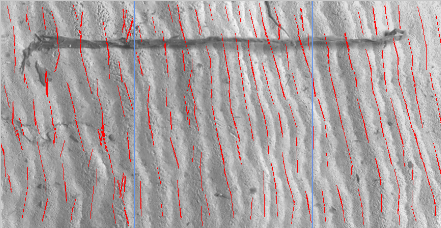
\includegraphics[width = 2.5in]{img/ManualUsuario/Cordillera}}
\subfloat{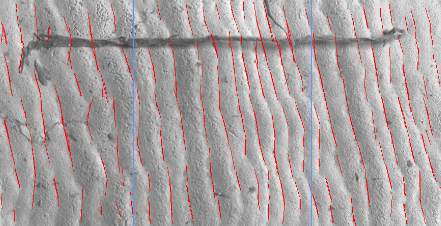
\includegraphics[width = 2.5in]{img/ManualUsuario/Valle}}
\caption[Opciones orientación de perikymata]{Opciones Vertical (izda.) y Vertical 2 (dcha.)}
\label{fig:PerikymataOrientation}
\end{figure}

Para terminar esta fase, comentaremos que también tenemos un botón \textit{Reset View} para volver a comenzar el proceso si los resultados no son los esperados. Este botón cargará la imagen recortada original.

\newpage
\subsection{Marcado de perikymata y exportación de datos}

Con la imagen ya filtrada pulsaremos el botón representado por un \textit{icono} de una línea. Pulsaremos y arrastraremos sobre la imagen pasando por las perikymata detectadas (color rojo) para que la aplicación pueda marcarlas posteriormente. También podemos ir pulsando sobre la imagen para que la línea se vaya creando. Si la línea excede los límites de la imagen, aparecerá un mensaje de error. El botón \textit{Clear Line} permite borrar la línea si no nos hemos equivocado.

Al pulsar el botón \textit{Auto-mark perikymata} se marcarán en verde las perikymata rojas por donde hemos pasado la línea (figura \ref{fig:img/ManualUsuario/FaseMarcado}). Es posible que algunos puntos verdes no sean verdaderamente una perikymata y otros puntos que se han quedado sin marcar sí; para ello disponemos en la esquina superior derecha de dos botones que nos permitirán añadir y quitar perikymata a la imagen. 

\imagenDos{img/ManualUsuario/FaseMarcado}{Marcado de perikymata}{1.02}

Una vez todo esté de nuestro gusto, pulsaremos el botón \textit{Export Data} y se guardará un fichero \textit{csv} en la carpeta del proyecto \textit{Perikymata\_Outputs}. Este archivo contendrá las perikymata marcadas, el decil en el que se encuentran, sus coordenadas en píxeles, y la distancia a la perikyma anterior.

\subsection{Otras funcionalidades}
En la parte superior de la ventana (figura \ref{fig:img/ManualUsuario/Menu}), tenemos tres menús con distintos botones, explicaremos los más relevantes.
\imagenDos{img/ManualUsuario/Menu}{Funcionalidades comunes}{0.35}

En el menú \textit{File} tenemos los siguientes botones:
\begin{itemize}
    \item \textit{New Proyect}: crea un nuevo proyecto en el que poder trabajar.
    \item \textit{Open Project}: permite abrir otros proyectos que tengamos.
    \item \textit{Save}: guarda el estado del proyecto.
    \item \textit{Close}: cierra la aplicación.
\end{itemize}

En el menú \textit{Configuration} tenemos:
\begin{itemize}
     \item \textit{Full Screen}: hace que la ventana de la aplicación se maximice. Es útil en etapas como la del filtrado y recuento de perikymata, pues permite ver mejor toda la interfaz.
      \item \textit{Set temporary folder}: para la unión de imágenes se necesita utilizar una carpeta sin rutas con espacios en blanco como carpeta temporal. Esta opción abre una ventana como la de la figura \ref{fig:img/ManualUsuario/CarpetaTemporal} para permitirnos seleccionar una carpeta temporal de nuestra elección. La aplicación mostrará un mensaje de error si se intenta seleccionar una carpeta con espacios en blanco en su ruta.
      
      \imagenDos{img/ManualUsuario/CarpetaTemporal}{Elección de carpeta temporal}{0.65}
\end{itemize}

En relación con este apartado, hay que explicar uno de los errores que se han encontrado al usar la aplicación en Linux. Puede darse la ocasión en que los botones de menú de la parte superior no respondan y que tampoco se pueda redimensionar la ventana. Salvo eso, la aplicación funciona con normalidad. Se desconoce el origen del error.


\subsection{Observaciones}

Sobre las imágenes a filtrar:\\
Las imágenes de fragmentos que se han proporcionado para este proyecto suelen venir incluidas en una carpeta. En ella encontramos imágenes con la leyenda que indica la medida y las mismas imágenes pero sin la leyenda. 

Para que las imágenes se puedan unir correctamente, es necesario que se escojan todas las imágenes sin leyenda menos una, para poder tomar la medida en la etapa correspondiente de la aplicación. Se recomienda que la imagen con la medida sea una de las esquinas, para interferir lo más mínimo con la operación de unión. Además, es labor del usuario que estas estén orientadas en el mismo sentido, de modo que las perikymata queden de forma vertical. Si al unir las imágenes obtenemos una imagen completamente negra, es posible que debamos eliminar de la lista alguna imagen muy similar a otra, porque esta puede comprometer la operación.

Sobre la aplicación en Linux y los scripts proporcionados:\\
Los usuarios de Windows pueden ver si funciona el servidor en una ventana de comandos, pero los usuarios de Linux no. Por eso en la carpeta \textit{PythonApp}, que contiene el servidor, se proporcionan los siguientes \textit{scripts} por si los usuarios encuentran dificultades para usar la aplicación por problemas del servidor:
\begin{itemize}
     \item \textit{StartServerLinux.sh}: enciende el servidor.
     \item \textit{StopServerLinux.sh}: detiene el proceso \textit{python3} que usa el servidor.
\end{itemize}

Para poder usarlos, habría que abrir una terminal dentro de la carpeta \textit{PythonApp} y escribir los siguientes comandos para cada \textit{script}. El primer comando solo es necesario la primera vez:\\
\centerline{\textit{\$ chmod +x script.sh}}
\centerline{\textit{\$ ./script.sh}}

Hay que comentar también, que los scripts están hechos para ejecutarse en una \textit{shell} de \textit{bash}, como la de Ubuntu, por ejemplo. Si se utiliza otra \textit{shell}, los usuarios pueden modificar los \textit{scripts} para adaptarlos.